\subsection{Bluetooth}
Bluetooth is a wireless technology standard for exchanging data over short distances (using short-wavelength UHF radio waves in the ISM band from 2.4 to 2.485 GHz from fixed and mobile devices, and building personal area networks (PANs). Invented by telecom vendor Ericsson in 1994, it was originally conceived as a wireless alternative to RS-232 data cables. It can connect several devices, overcoming problems of synchronization.\\
Bluetooth is managed by the Bluetooth Special Interest Group (SIG), which has more than 25,000 member\cite{bluetooth}companies in the areas of telecommunication, computing, networking, and consumer electronics. The IEEE standardized Bluetooth as IEEE 802.15.1, but no longer maintains the standard. The Bluetooth SIG oversees development of the specification, manages the qualification program, and protects the trademarks.A manufacturer must make a device meet Bluetooth SIG standards to market it as a Bluetooth device. A network of patents apply to the technology, which are licensed to individual qualifying devices.
\subsubsection{Bluetooth Implementation}
Bluetooth operates at frequencies between 2402 and 2480 MHz, or 2400 and 2483.5 MHz including guard bands 2 MHz wide at the bottom end and 3.5 MHz wide at the top. This is in the globally unlicensed Industrial, Scientific and Medical (ISM) 2.4 GHz short-range radio frequency band. Bluetooth uses a radio technology called frequency-hopping spread spectrum.\\
 Bluetooth is a packet-based protocol with a master-slave structure. One master may communicate with up to seven slaves in a piconet. All devices share the master's clock. Packet exchange is based on the basic clock, defined by the master.\\
A master Bluetooth device can communicate with a maximum of seven devices in a piconet (an ad-hoc computer network using Bluetooth technology), though not all devices reach this maximum. As in our project the Bluetooth module HC-05 is only able to communicate to just one connected device. The devices can switch roles, by agreement, and the slave can become the master.
\subsubsection{Communication and connection}
A master Bluetooth device can communicate with a maximum of seven devices in a piconet (an ad-hoc computer network using Bluetooth technology), though not all devices reach this maximum. The devices can switch roles, by agreement, and the slave can become the master (for example, a headset initiating a connection to a phone necessarily begins as master—as initiator of the connection—but may subsequently operate as slave).\\
The Bluetooth Core Specification provides for the connection of two or more piconets to form a scatternet, in which certain devices simultaneously play the master role in one piconet and the slave role in another.\\
At any given time, data can be transferred between the master and one other device (except for the little-used broadcast mode.[citation needed]) The master chooses which slave device to address; typically, it switches rapidly from one device to another in a round-robin fashion. Since it is the master that chooses which slave to address, whereas a slave is (in theory) supposed to listen in each receive slot, being a master is a lighter burden than being a slave. Being a master of seven slaves is possible; being a slave of more than one master is difficult.[citation needed] The specification is vague as to required behavior in scatternets.
\subsubsection{Bluetooth Architecture}
The Bluetooth architecture\cite{bluetooth2} is shown below:
\begin{figure}[htp]
\center
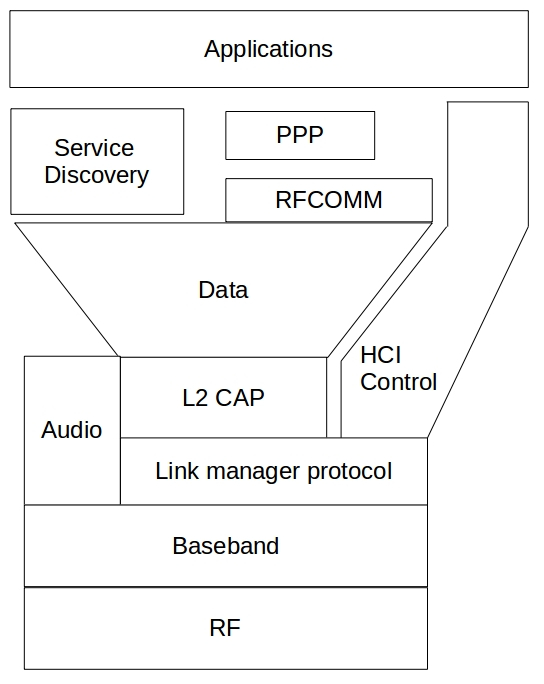
\includegraphics[scale=0.5]{bluetootharchitecturenew.jpg}  
\caption{Bluetooth Architecture}
\end{figure}
\subsubsection{Bluetooth Topology}
There can be only 2 - 7 Bluetooth devices talking to each other. This is called a piconet. Among these devices, there can be only one master device, all the rest are slave devices. A device can belong to two piconets meantime, serving as slaves in both piconet or a master in one and slave in another. This is called a bridging device. Bridging devices connect piconets together to form a scatternet:\cite{bluetooth2}
\begin{figure}[htp]
\center
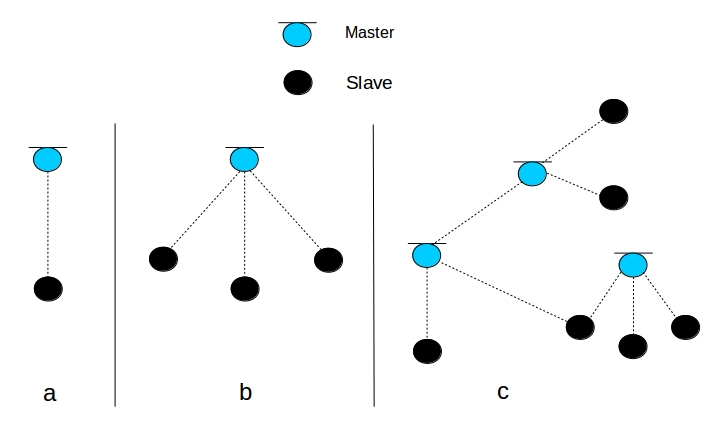
\includegraphics[scale=0.5]{topology.jpg} 
\caption{Single-slave piconet (a), multiple-slave piconet(b) and scatternet (c)}
\end{figure}
\subsubsection{RF and Baseband}
\subsubsection*{RadioFrequency}
Bluetooth operates at the unlicensed 2.5GHz Industrial-Scientific-Medical (ISM) band. There are already many types of devices using this band, such as baby monitors and garage door remote controls. To avoid interfering with these devices, Bluetooth devices sends out very weak signals (about 1 milliwatt). This limits the transmission range to 10 meters. It also uses a frequency hopping technique, hopping randomly between 79 1-MHz channels 1600 times per second (625 us time slot). Each piconet is synchronized to a specific frequency hopping pattern\cite{bluetooth2}, so that even different piconets do not interfere with each other. A piconet can either be static or dynamic (chaning when devices move in or out).
\subsubsection*{Modulation in Bluetooth}
The modulation in Bluetooth is Gaussian Frequency Shift Keying\cite{bluetooth2}(GFSK), with a BT = 0.5 and modulation index between 0.25 and 0.35.
Gaussian frequency shift keying (GFSK) is a modulation method for digital communication found in many standards such as Bluetooth, DECT and Wavenis. Digital communication amounts to translating symbols from a discrete alphabet into a signal that the transmitting side can send into a transmission medium and from which the receiving side can recover the original symbols.
\begin{figure}[h]
\center
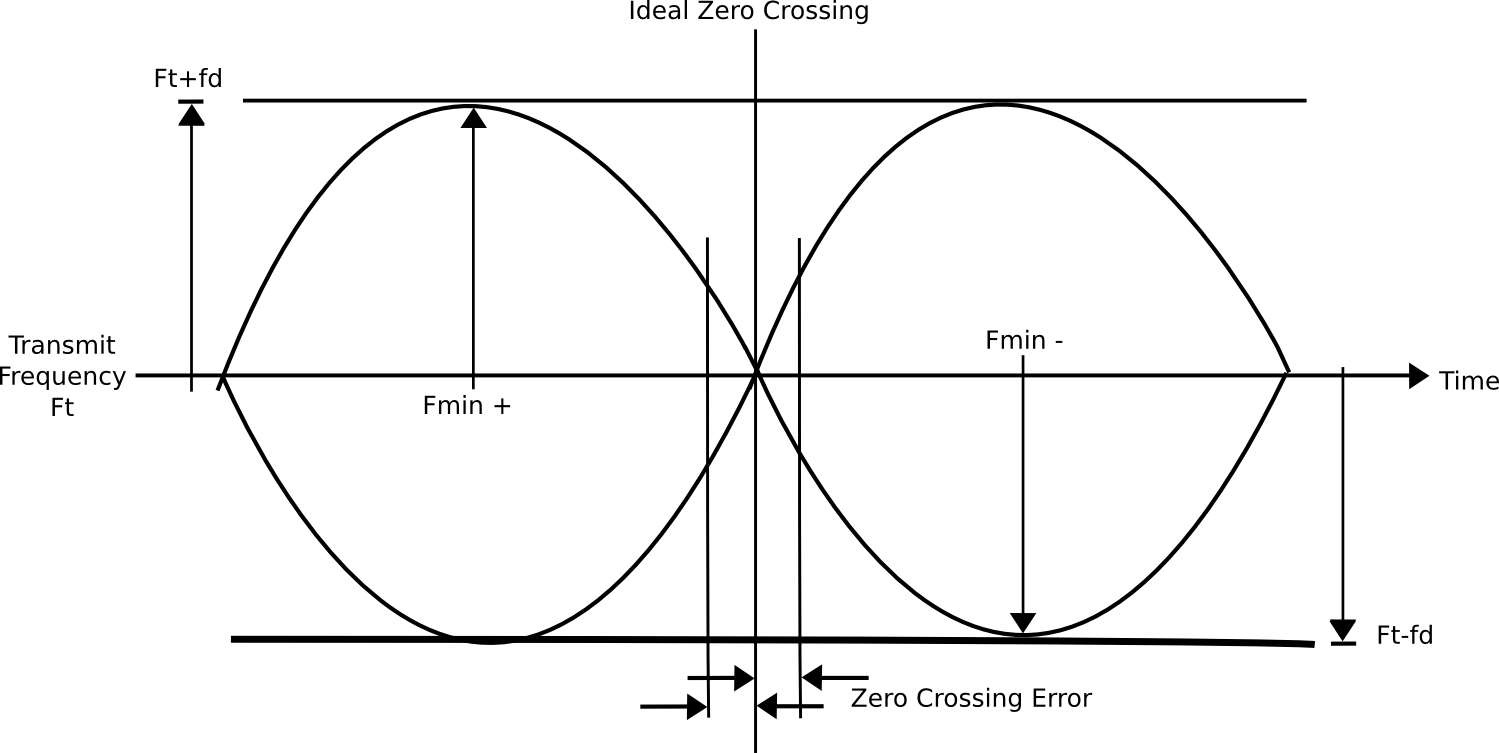
\includegraphics[scale=01]{sinewave.png}  
\caption{GFSK Modulation in Bluetooth}
\end{figure}
\subsubsection{Packet Format}
Data in piconet is encoded in packets. The general packet format is shown below:
\begin{figure}[h]
\center
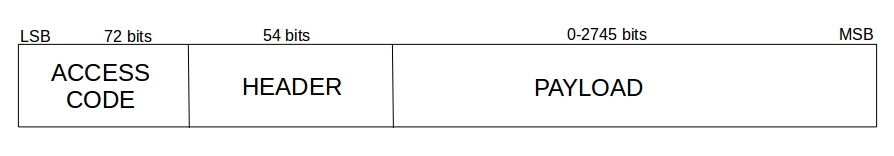
\includegraphics[scale=0.5]{first.jpg} 
\caption{General Packet Format of Bluetooth}
\end{figure}
\subsubsection*{Access Code}
Access code is used for synchronization, DC offset compensation and identification.
\subsubsection*{Header}
Header part of the packet is used by the Link Control (LC) logical channel. It has the following format:
\begin{figure}[h]
\center
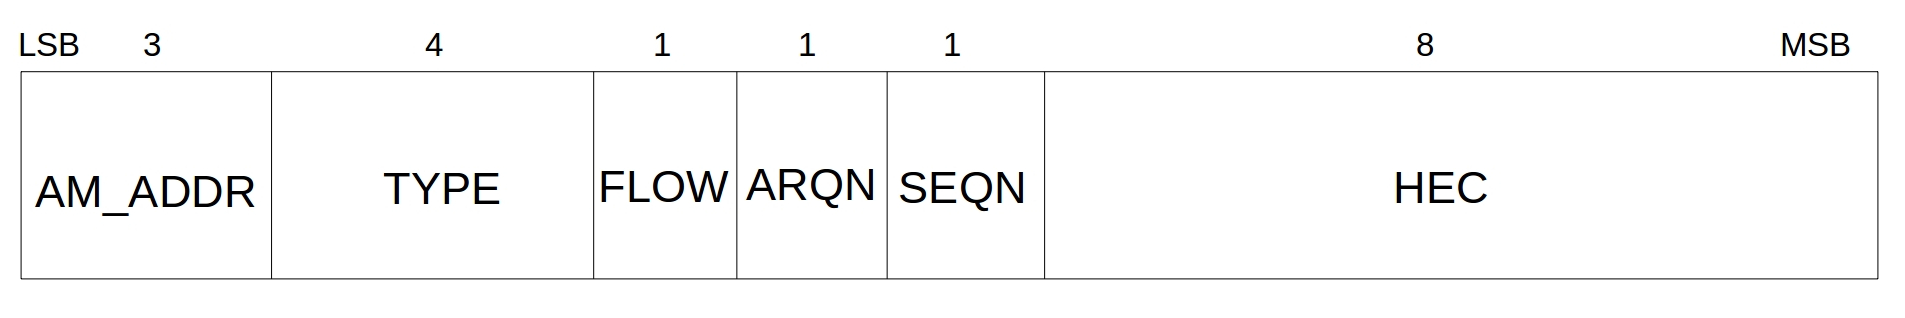
\includegraphics[scale=0.2]{second.jpg}
\caption{Header Format of Bluetooth Packet}
\end{figure}
\subsubsection*{Payload}
There can be two types of payload: voice and data. Synchronous Connection-Oriented(SCO) packets only have voice field, while Asynchronous Connectionless(ACL) packets only have data field.
\subsubsection{Physical Links}
Bluetooth protocol uses a combination of synchronous and asynchronous links. A Synchronous Connection-Oriented (SCO) link is a point-to-point link between the master and specific slave. It has symmetric 64 kbps rate, typically used for voice transmission. It uses reserved time slots, thus can be regarded as a circuit switching link. A master can support up to 3 SCO links to one or multiple slaves, while a slave can support up to three SCO links to one master or up to two SCO links to different masters. Master transmits at reserved master-to-slave time slot, and slave response in the following slave-to-master slot. SCO packets are never retransmitted.\\
Asynchronous Connectionless (ACL) links are used for data transmission, with 723.2 downstream/57.6 kbps upstream asymmetric or 433.9 kbps symmetric data rate. There can be only one ACL link between the master and all active slaves. Only the addressed slave device can response. ACL packets can be retransmitted for data integrity.
\subsection{Serial Communication}
Serial data transfer is when we transfer data one bit at a time, one right after the other. These
interfaces can operate on as little as one wire, usually never more than four.
Asynchronous mode of data transfer means that data is transferred without support from an
external clock signal. This transmission method is perfect for minimizing the required wires
and I/O pins, but it does mean we need to put some extra effort into reliably transferring and
receiving data. The asynchronous serial protocol has a number of built-in rules or
mechanisms that help ensure robust and error-free data transfers.
\subsubsection{Baud Rate}
The baud rate specifies how fast data is sent over a serial line. It’s usually expressed in units
of bits-per-second (bps) provided each signal transition represents a data transfer. If you
invert the baud rate, you can find out just how long it takes to transmit a single bit. This
value determines how long the transmitter holds a serial line high/low or at what period the
receiving device samples its line.\\
Baud rates can be just about any value within reason. The only requirement is that both
devices operate at the same rate. One of the more common baud rates, especially for simple
stuff where speed isn’t critical, is 9600 bps. Other “standard” baud are 1200, 2400, 4800,
19200, 38400, 57600, and 115200.
\subsubsection{Synchronization bits}
The synchronization bits are two or three special bits transferred with each chunk of data.
They are the start bit and the stop bit(s). There’s always only one start bit, but the number of
stop bits is configurable to either one or two. The start bit is always indicated by an idle data
line going from 1 to 0, while the stop bit(s) will transition back to the idle state by holding
the line at 1.
\subsubsection{Parity Bits}
Parity is a form of very simple, low-level error checking. It comes in two flavors: odd or
even. To produce the parity bit, all 5-9 bits of the data byte are added up, and the evenness
of the sum decides whether the bit is set or not. For example, assuming parity is set to even
and was being added to a data byte like 0b01011101, which has an odd number of 1’s (5),
the parity bit would be set to 1. Conversely, if the parity mode was set to odd, the parity bit
would be 0. Parity is optional, and not very widely used. It can be helpful for transmitting
across noisy mediums, but it’ll also slow down your data transfer a bit and requires both
sender and receiver to implement error-handling.\begin{table}[h]
\begin{center}
\begin{tabular}{ |c|c|c|c|c| } 
 \hline
 FRAME:& Start& Data &Parity& Stop\\
\hline 
SIZE (BITS):& 1& 5-9& 0-1& 1-2\\
\hline
\end{tabular}
\caption{Serial Frame}
\end{center}
\end{table}
